\section{Hyperparameter von DPSGD}\label{sec:hyperparams}

Die Güte eines Modells wird durch die Wahl der Hyperparameter beeinflusst. 
Dies gilt sowohl beim normalen Training, als auch beim Training mit DPSGD.
Im Folgenden wird getestet, welche Parameter die Güte eines neuronalen Netzes bei der Nutzung von DPSGD beeinflussen.
Dazu werden die drei Modelle, welche in Kapitel \ref{sec:use_case} beschrieben wurden, mit verschiedenen Hyperparametern trainiert und evaluiert.
Dabei werden DPSGD spezifische Parameter, wie der $\epsilon$-Wert und die Clipping-Norm, und auch allgemeine Parameter, wie die Batch-Größe und die Anzahl der Epochen, betrachtet.
Die Lernrate wird dabei nicht konstant festgelegt, sondern über den \textbf{Adam}-Optimizer in PyTorch adaptiv konfiguriert.
Der Adam-Optimizer passt die Lernrate anhand des Momentums und der Varianz der Gradienten an \cite{adam}.

Bevor das eigentliche Modell trainiert wird, gibt es die Möglichkeit, die Datenmenge per Datenaugmentierung, auch Data Augmentation genannt, künstlich zu erweitern.
Bei Bildern können die Werte einzelner Pixeln beeinflusst werden, indem der Farbraum der Bilder angepasst wird, oder Kontraste erhöht werden.
Zusätzlich können Bilder über Rotation und Spieglung transformiert werden.
Dabei können die Werte der Anpassung, \zB die Verstärkung des Kontrasts, konfiguriert werden und an eine Wahrscheinlichkeit geknüpft werden.
PyTorch bietet über AutoAugment eine Möglichkeit an, eine Kombination verschiedener Anpassungen zu nutzen \cite{autoaugment}.
Die Nutzung von AutoAugment, sowie dessen Einfluss auf die Güte der Modelle, wird folglich mitberücksichtigt.

Da das CIFAR-10 Modell die geringste Anzahl an lernbaren Parameter besitzt, wird die Anpassung verschiedener Parameter an diesem Modell zuerst evaluiert.
Anschließend werden die Erkenntnisse auf das ResNet-18 Modell und das Vision Transformer Modell für den CelebA Datenbestand angewendet.
Im Folgenden werden einige Auszüge aus den gesamten Ergebnissen zur Veranschaulichung herangezogen. 
Die vollständigen Tabellen aller Messwerte befinden sich in Anhang \ref{ch:ergebnisse_detail}.

\subsection{Hyperparameter CIFAR-10 Modell}

Für das CIFAR-10 Modell, welches kein DPSGD nutzt, werden folgende Hyperparameter betrachtet: Anzahl der Epochen, Batch-Größe und die Nutzung von AutoAugment.
Dazu wurde das Modell mit einer Epochenanzahl zwischen 10 und 20 trainiert, jeweils mit einer Batch-Größe von 64, 128 oder 256. 
Dieser Vorgang wurde mit AutoAugment aktiviert und deaktiviert ausgeführt.
Die höchste Genauigkeit wird erreicht, wenn das Modell mit Datenugmentierung und einer Batch-Größe von 64 über 15 Epochen hinweg trainiert wird.
Die erreichte Genauigkeit, welche anhand der Test-Daten gemessen wurde, liegt bei 84,6 \%.

Eine Batch-Größe von 64 und 128 resultieren in einer ähnlichen Güte des Modells. 
Jedoch sorgt eine Batch-Größe von 256 für eine geringere Genauigkeit des Modells. 
Dies liegt daran, dass einzelne Datensätze in der Aggregation der Gradienten untergehen können, wodurch einzelne Features der Daten weniger gut gelernt werden. 
Abbildung \ref{fig:cifar-1} zeigt die Güte der Modelle, welche mit den unterschiedlichen Batch-Größen trainiert wurden.
Jede Linie steht dabei für eine unterschiedliche Anzahl an trainierten Epochen.
\begin{figure}[!htb]
    \centering
    \fbox{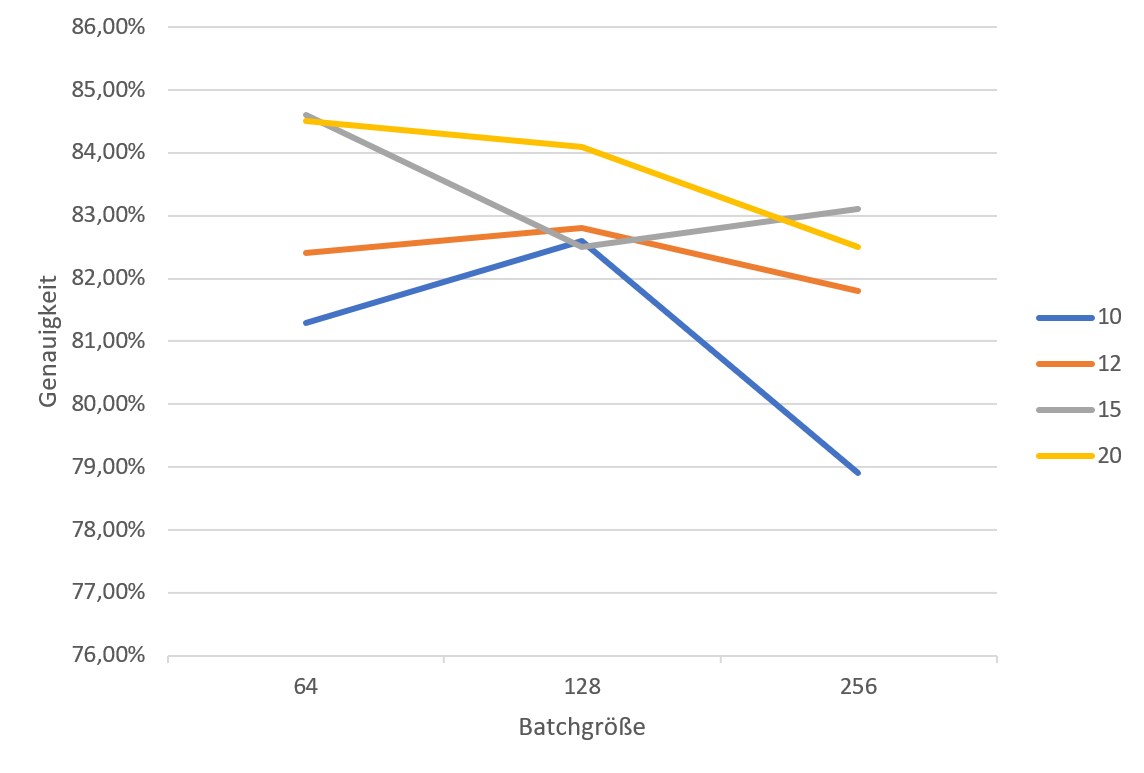
\includegraphics[width=14cm]{figures/results_cifar/cifar_batch_base.png}}
    \caption{Auswirkung Batch-Größe auf CIFAR-10 Modell ohne DPSGD und mit \\Datenaugmentierung}
    \label{fig:cifar-1}
\end{figure} 

Zusätzlich zeigt Abbildung \ref{fig:cifar-1}, dass eine höhere Anzahl an Epochen mit einer höheren Genauigkeit korreliert.
Dies liegt an der Nutzung von Datenaugmentierung. 
Wird diese nicht genutzt, liegt die optimale Anzahl an Epochen zwischen 12 und 15. 
Werden mehr Epochen trainiert, sinkt die Genauigkeit wieder, was auf ein Overfitting des Modells zurückzuführen ist.
Generell sinkt die Genauigkeit der Modelle, wenn AutoAugment nicht genutzt wird. 
Durch die Datenaugmentierung wird der Datensatz künstlich erweitert, was dafür sorgt, dass die Trainingsdatenmenge vergrößert wird.

Für das CIFAR-10 Modell ohne DPSGD resultieren folgendende Hyperparameter in einer optimalen Güte des Modells:
\begin{compactitem}
    \item \textbf{Batch-Größe:} Batch-Größe kann variablen gewählt werden, sollte jedoch nicht zu groß sein. Ein Wert von 64 oder 128 ist wirksam.
    \item \textbf{Anzahl Epochen:} Die optimale Anzahl an Epochen ist um 15 herum. Wird Datenaugmentierung genutzt, kann die Anzahl höher sein, wenn nicht, dann sollte die Anzahl geringer sein.
    \item \textbf{Datenaugmentierung:} Datenaugmentierung verbessert die Güte des Modells und ermöglicht das Training mehrerer Epochen, wobei Overfitting vermieden wird. Datenaugmentierung sollte deshalb genutzt werden.
\end{compactitem}


Wird das CIFAR-10 Modell mit DPSGD trainiert, müssen zusätzlich noch der $\epsilon$-Wert des Privacy Budgets und die Clipping-Norm betrachtet werden. 
Der $\delta$-Wert des Privacy Budgets wird konstant auf $10^{-5}$ festgelegt.
Um die Hyperparameter zu evaluieren, gibt es drei unterschiedliche Versuche.
Alle drei Versuche trainieren eine Vielzahl an Modellen mit DPSGD.
Dabei werden $\epsilon$-Werte von 1 bis 50, Epochenanzahlen von 1 bis 30 und Batch-Größen von 64 bis 256 genutzt.
Lediglich bei der Clipping-Norm und bei der Nutzung von Datenaugmentierung unterscheiden sich die drei Versuche.
Um den festgelegten $\epsilon$-Wert nach einer festgelegten Anzahl an Epochen zu erreichen, wurde die \textit{\mbox{make\_private\_with\_epsilon()}}-Methode genutzt.

Der erste Versuch nutzt Datenaugmentierung und hat einen nicht optimierten Wert der Clipping-Norm.
Dieser ist auf 1,0 festgelegt.
Dieser Versuch zeigt, dass die Genauigkeit der Modelle, mit der Größe des $\epsilon$-Werts zunimmt.
Bei einem $\epsilon$-Wert von 1 wird maximal eine Genauigkeit von 36,9 \% erreicht, wohingegen bei einem $\epsilon$-Wert von 50 eine Genauigkeit von 59,1 \% erreicht wird.
Ebenfalls steigt die Genauigkeit der Modelle mit der Anzahl an trainierten Epochen. 
Dies liegt daran nicht nur daran, dass Datenaugmentierung genutzt wird, sondern dass auch das Rauschen Overfitting verhindert.
Sogar 30 Epochen können trainiert werden, ohne dass die Genauigkeit stagniert.
Anders als bei dem Modell ohne DPSGD, hat die Batch-Größe eine deutliche Auswirkung auf die Genauigkeit der Modelle.
Eine höhere Batch-Größe sorgt für eine verbesserte Genauigkeit der Modelle.
Das Rauschen, welches den einzelnen Gradienten hinzugefügt wird, gleicht sich bei einer höheren Batch-Größe aus und nähert sich dem Erwartungswert an. 
Da der Erwartungswert den echten Gradienten entspricht, bedeutet dies, dass eine höhere Batch-Größe dafür sorgt, dass die verrauschten Gradienten der Gewichte, näher an den tatsächlichen Gradienten der Gewichte liegen.
Abbildung \ref{fig:cifar-2} zeigt diesen Zusammenhang grafisch.
Jede Linie entspricht einem Modell, welches über 15 Epochen, mit unterschiedlichem $\epsilon$-Wert, trainiert wird.
\begin{figure}[!htb]
    \centering
    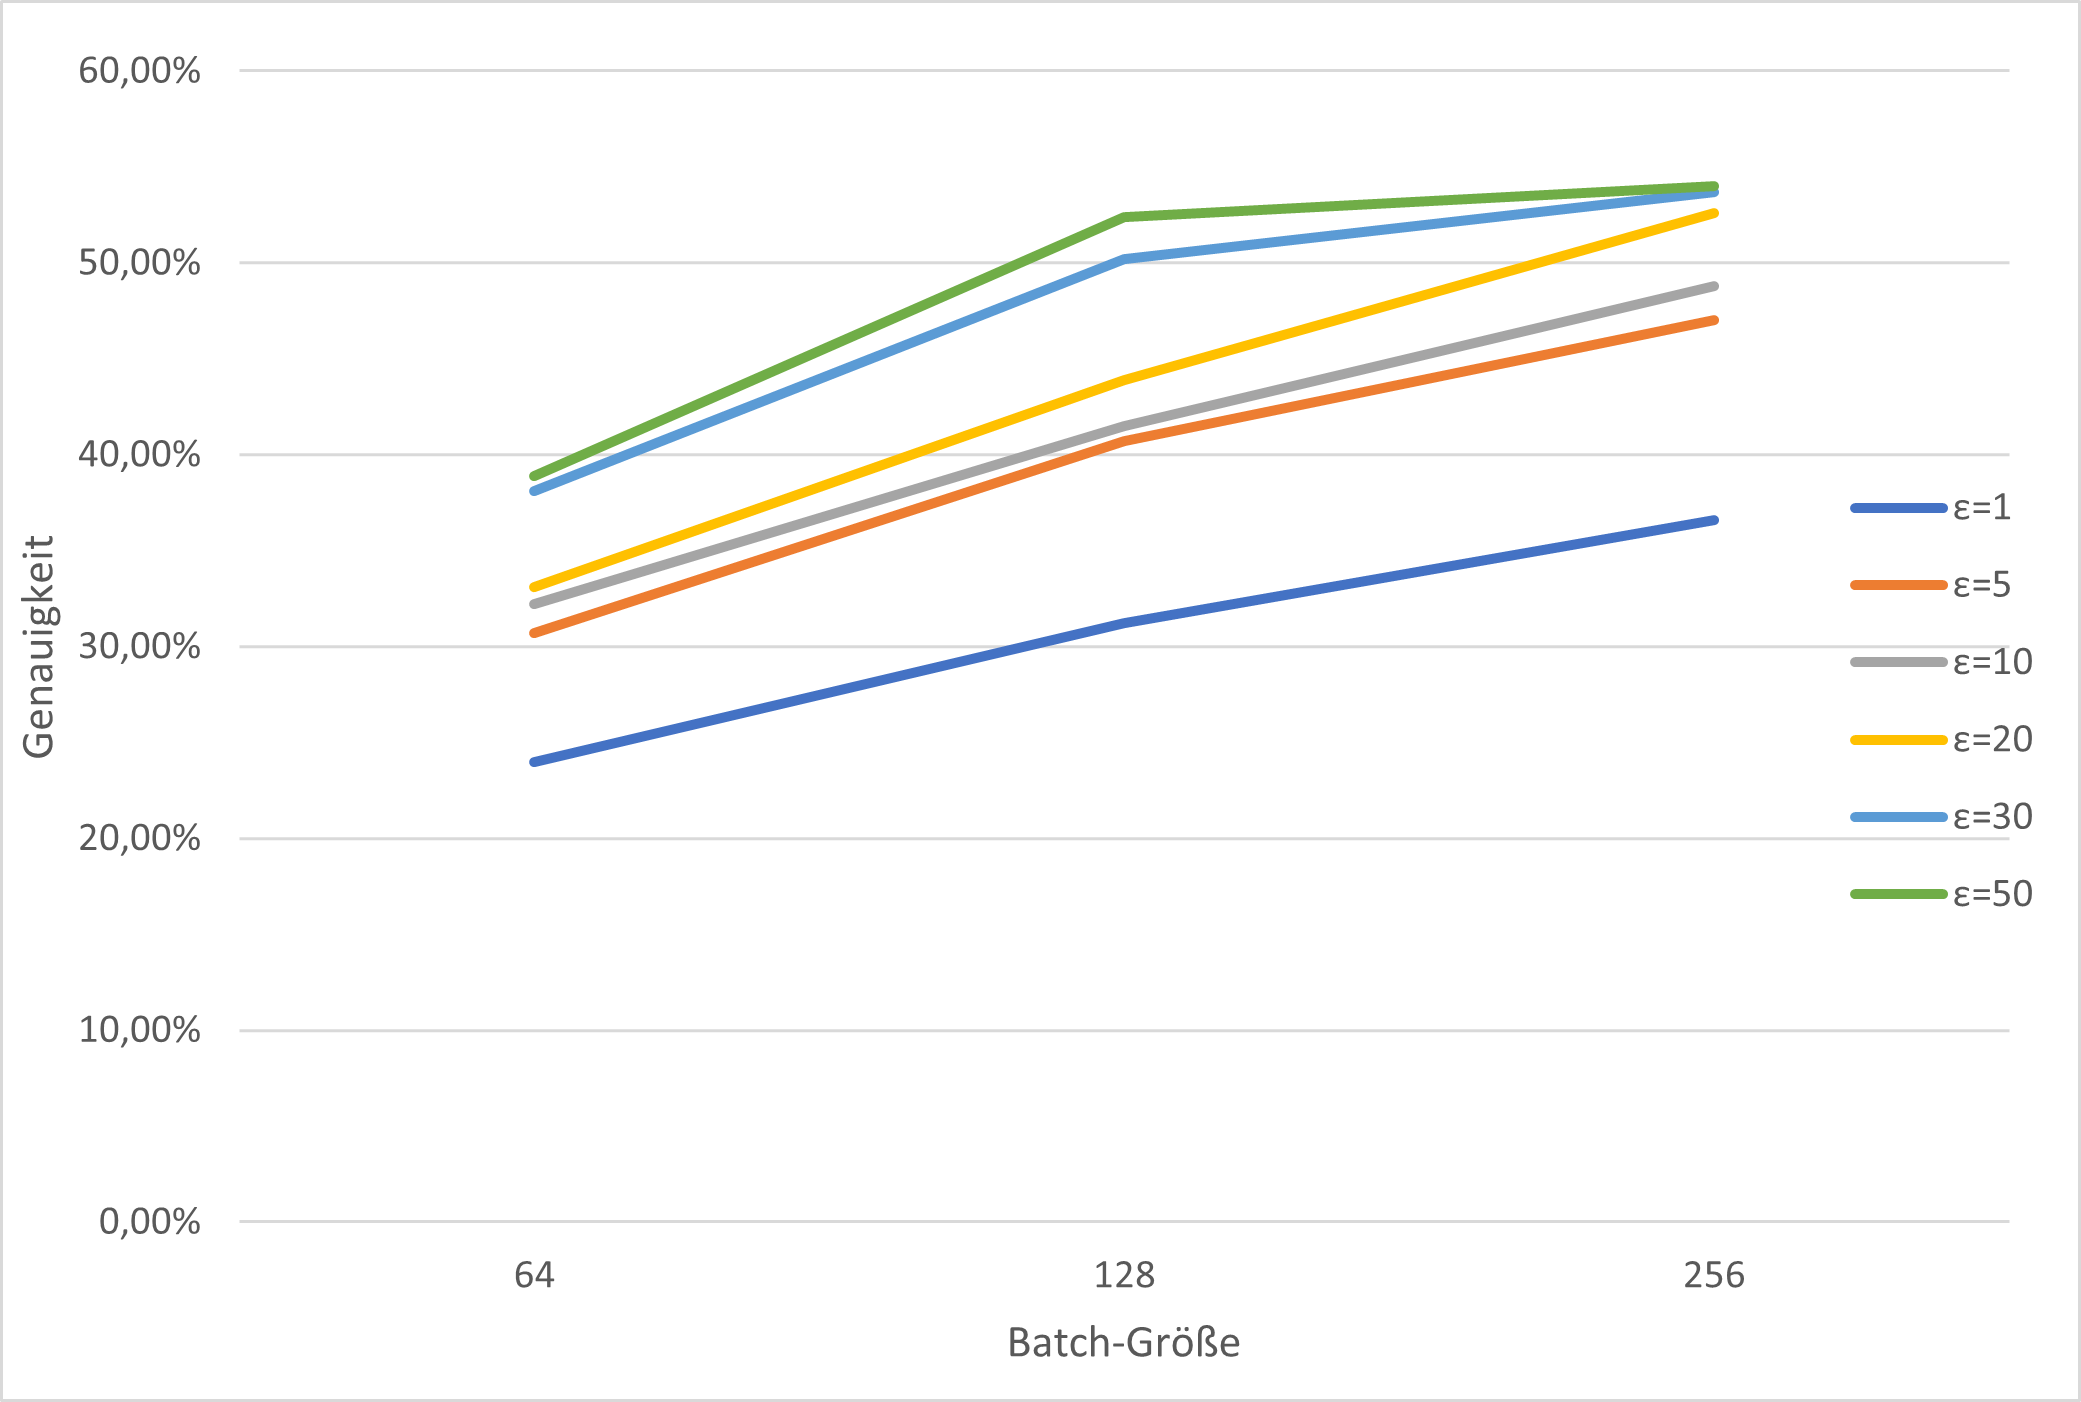
\includegraphics[width=14cm]{figures/results_cifar/cifar_batch_1.png}
    \caption{Auswirkung der Batch-Größe auf die Genauigkeit von CIFAR-10 Modellen}
    \label{fig:cifar-2}
\end{figure} 

Der zweite Versuch ähnelt dem ersten Versuch, jedoch wird die Datenaugmentierung nicht genutzt.
Dies sorgt dafür, dass die Genauigkeit der Modelle steigt. 
Abbildung \ref{fig:cifar_aug3} zeigt diesen Zusammenhang.
Die Modelle, dessen Genauigkeit dargestellt werden, werden jeweils 15 Epochen lang, mit einer Batch-Größe von 256, trainiert.
\begin{figure}[!htb]
    \centering
    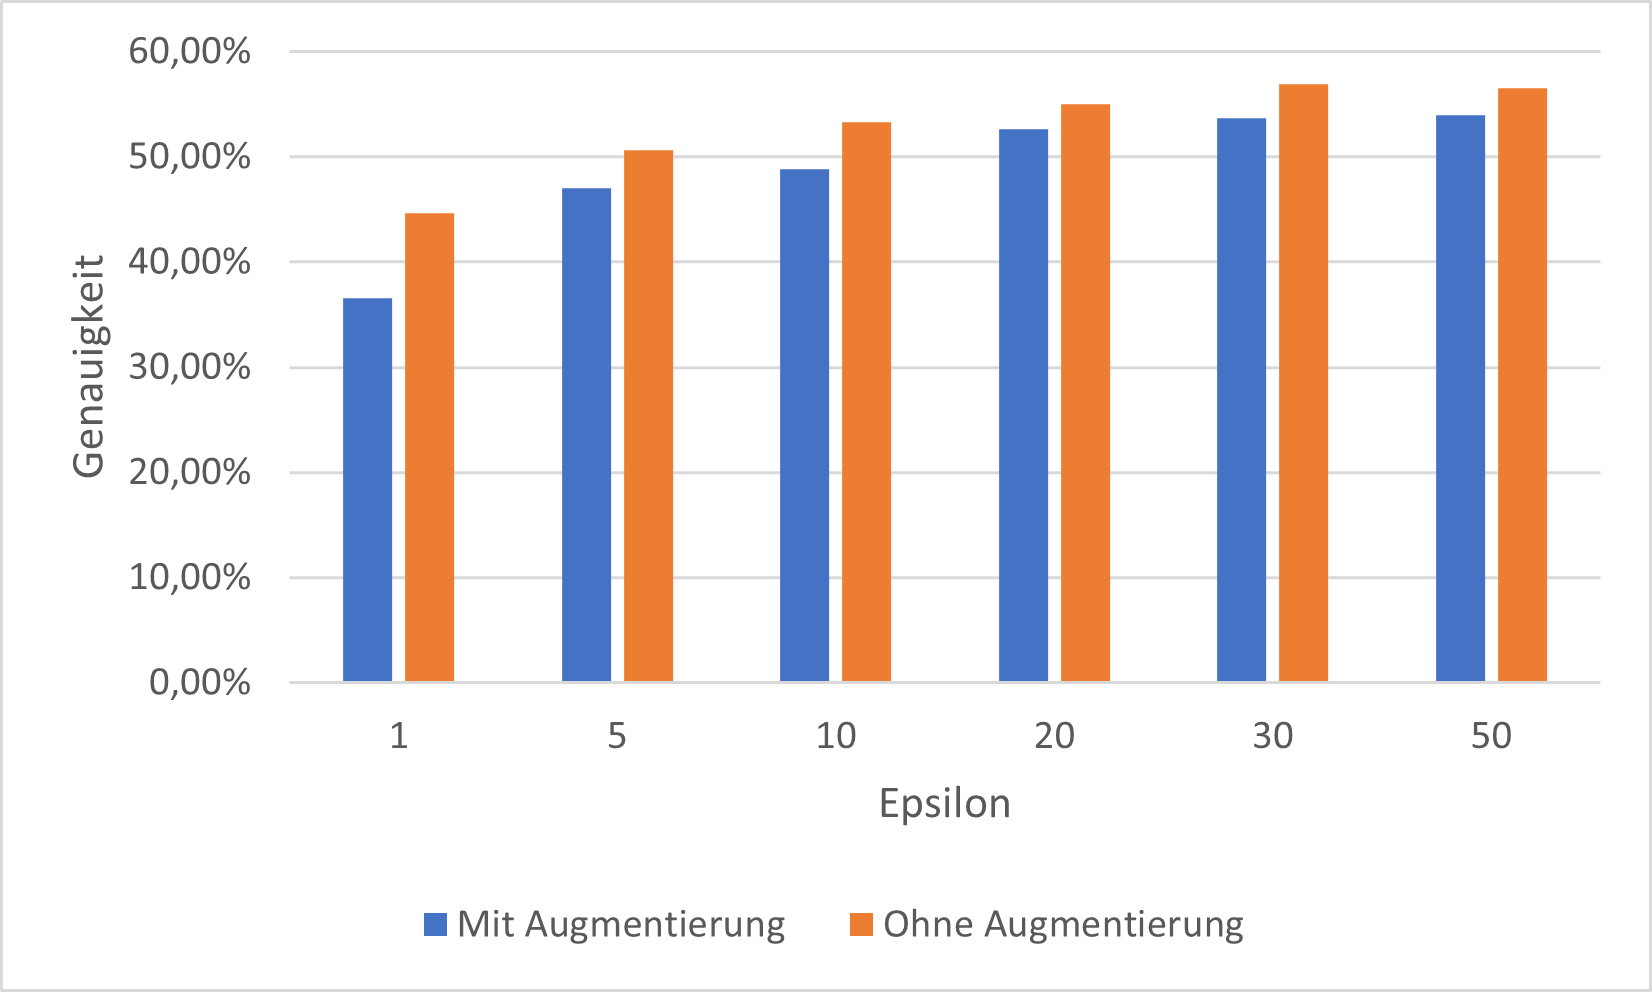
\includegraphics[width=14cm]{figures/results_cifar/cifar_aug3.png}
    \caption{Auswirkung von AutoAugment auf die Genauigkeit von CIFAR-10 Modellen}
    \label{fig:cifar_aug3}
\end{figure} 
Obwohl die Datenaugmentierung im zweiten Versuch nicht genutzt wird, kann das Modell 20 Epochen lang trainiert werden und hat dennoch eine steigende Genauigkeit.
Erst im Bereich zwischen 20 und 30 Epochen stagniert die Genauigkeit.
Im Vergleich zu dem Modell ohne DPSGD sind dies dennoch einige Epochen mehr.
Dies liegt daran, dass das Rauschen, genau wie die Datenaugmentierung, das Overfitting reduziert.

Der dritte Versuch gleicht dem zweiten Versuch, wobei hier der Wert der Clipping-Norm angepasst wurde.
Da die Clipping-Norm die Stärke des Rauschens beeinflusst, kann ein geringer Wert die Güte eines Modells erhöhen.
Wird der Wert jedoch zu gering gewählt, kann dies auch für den gegenteiligen Effekt sorgen, denn die Gradienten werden zu klein, damit das Modell in den geplanten Trainingsschritten konvergiert.
Um eine geeignete Clipping-Norm zu finden, wird das CIFAR-10 Modell über 5 Epochen trainiert, ohne Rauschen, jedoch mit unterschiedlichen Werten für das Clipping.
Dabei werden Zehnerpotenzen genutzt.
Der Wert wird immer um eine Zehnerpotenz reduziert, solange bis das Clipping einen leichten negativen Einfluss auf die Güte des Modells hat.
Die resultierende Zehnerpotenz ist in diesem Fall $10^{-5}$.
Da diese einen leichten negativen Einfluss auf das Modell hat, bedeutet dies, dass eine Vielzahl an Gradienten durch diesen Wert begrenzt wird.
Die Wahl der Clipping-Norm sollte auf diesen Wert fallen, oder einen minimal höheren Wert, welcher keinen Einfluss auf das Modell hat.
Durch die Wahl dieses geringen Werts wird auch die Stärke des Rauschens reduziert.
In diesem dritten Versuch wird die Clipping-Norm von $10^{-5}$ evaluiert.

Die Anpassung der Clipping-Norm wirkt sich nicht bei einer niedrigen Anzahl an Epochen aus.
Bei den CIFAR-10 Modellen, welche 15 Epochen lang trainiert werden, ist die Genauigkeit in etwa gleich, egal ob die Clipping-Norm bei 1 oder bei $10^{-5}$ liegt. 
Abbildung \ref{fig:cifar_clip1} zeigt den soeben beschriebenen Zusammenhang.
\begin{figure}[!htb]
    \centering
    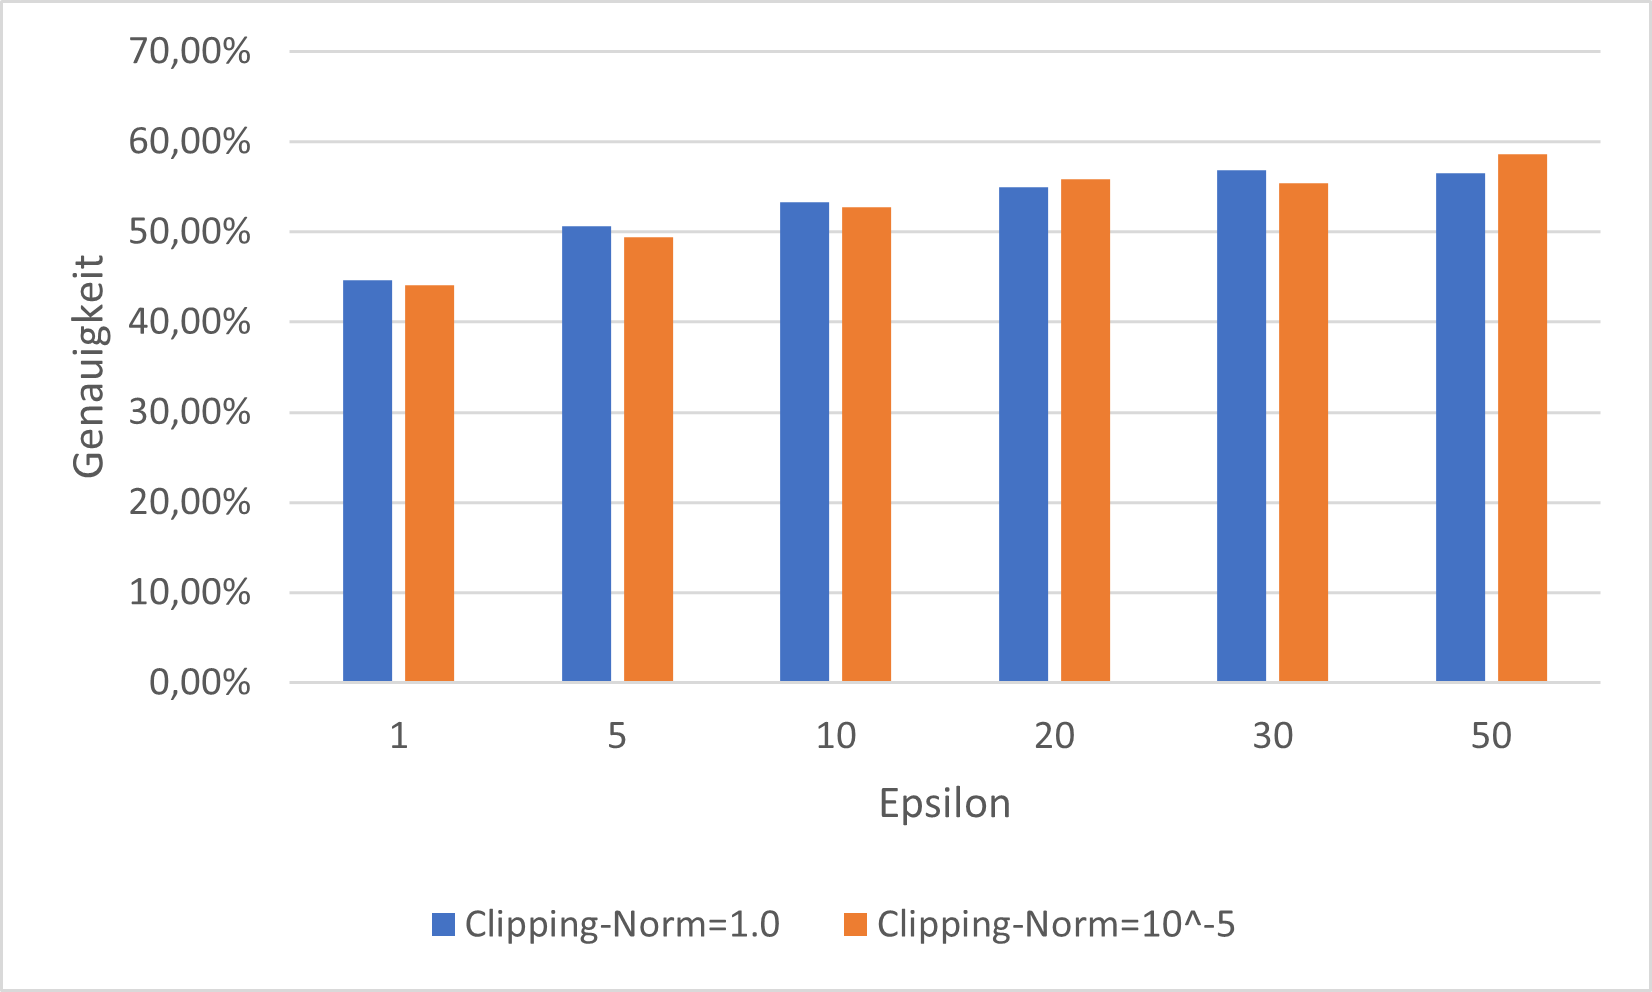
\includegraphics[width=14cm]{figures/results_cifar/cifar_clipp1.png}
    \caption{Auswirkung der Clipping-Norm auf die Güte von CIFAR-10 Modellen bei 15 Epochen Training}
    \label{fig:cifar_clip1}
\end{figure} 

Jedoch ermöglicht die geringere Clipping-Norm, mehr Epochen zu trainieren, ohne dass die Genauigkeit der Modelle stagniert. 
Dies liegt daran, dass die Gradienten mit kleiner Clipping-Norm kleiner sind, als die Gradienten mit großer Clipping-Norm. 
Somit werden mehr Trainingsschritte benötigt, um zu konvergieren. 
Außerdem ist die Stärke des Rauschens geringer, was ebenfalls die Güte des Modells verbessert.
Abbildung \ref{fig:cifar_clip2} zeigt den Vergleich zwischen einer hohen und einer niedrigen Clipping-Norm, wenn die Modelle jeweils 30 Epochen trainiert werden.

\begin{figure}[!htb]
    \centering
    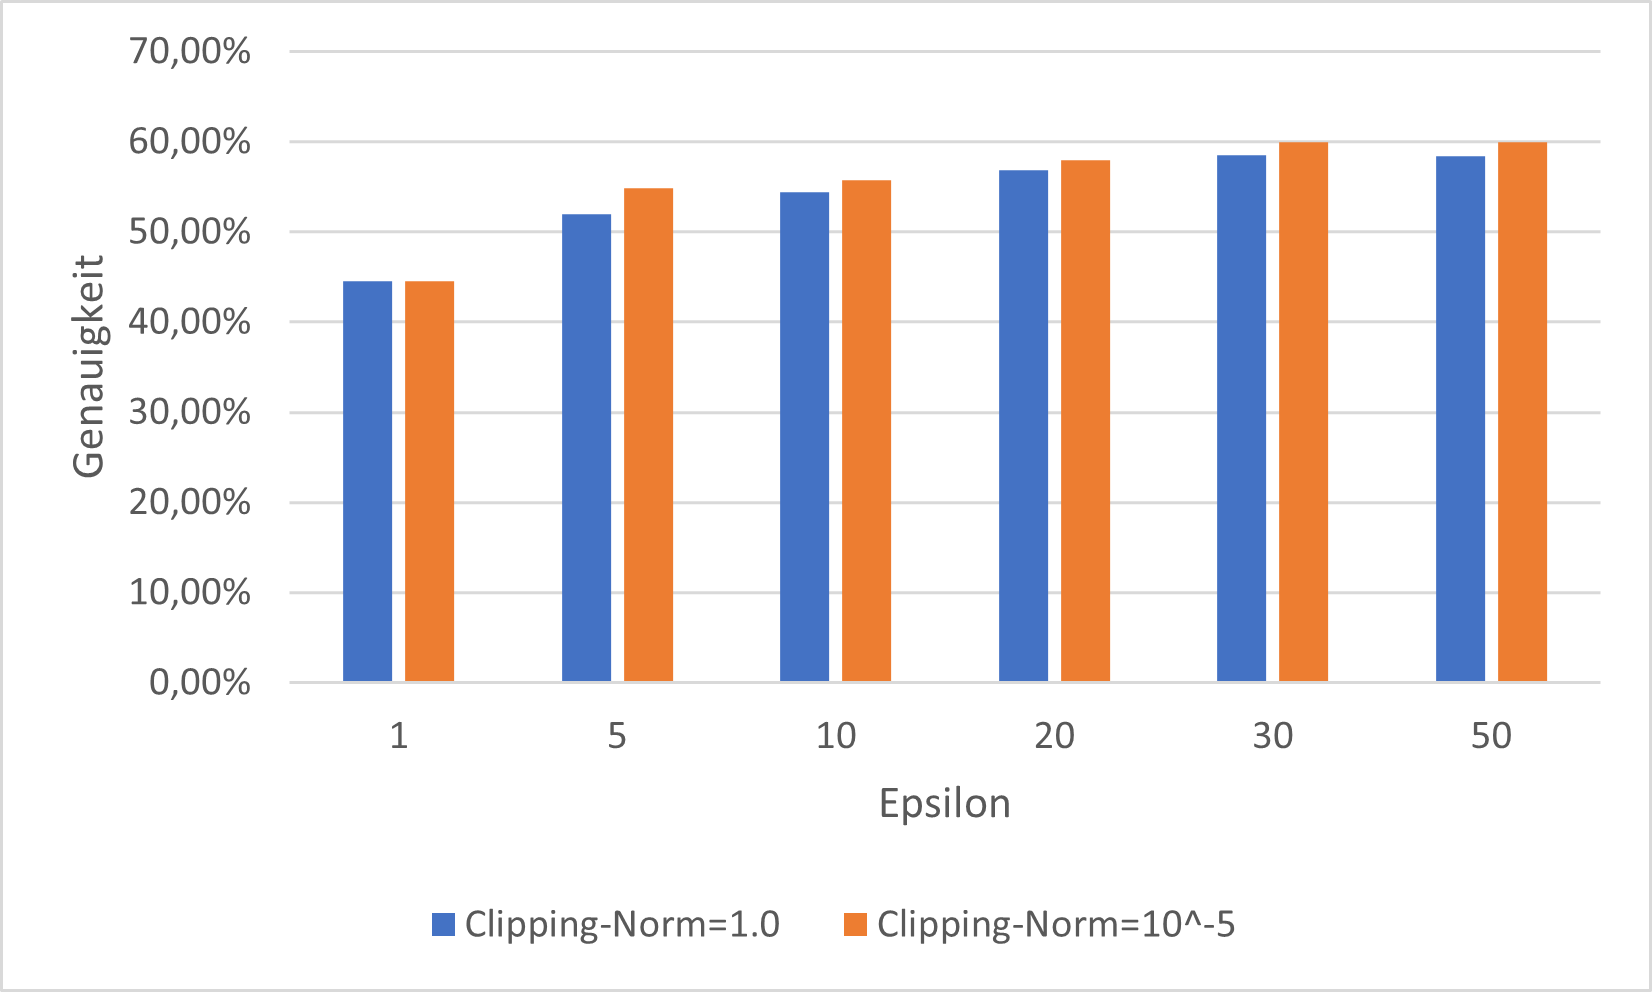
\includegraphics[width=14cm]{figures/results_cifar/cifar_clipp2.png}
    \caption{Auswirkung der Clipping-Norm auf die Güte von CIFAR-10 Modellen bei 30 Epochen Training}
    \label{fig:cifar_clip2}
\end{figure} 


Für das CIFAR-10 Modell mit DPSGD resultieren folgende Hyperparameter in einer optimalen Güte des Modells:
\begin{compactitem}
    \item \textbf{$\epsilon$-Wert des Privacy Budgets:} Der $\epsilon$-Wert korreliert mit der Güte des Modells. Kleine Werte schränken die Genauigkeit der Modelle ein, können aber die Vertraulichkeit besser schützen. Kapitel \ref{sec:bw_dp} gibt dabei einen Überblick über den Schutz der Modelle.
    \item \textbf{Batch-Größe:} Die Batch-Größe sollte möglichst groß gewählt werden. Hier kann ebenfalls der BatchMemoryManager von Opacus helfen, welcher eine virtuelle Batch-Größe ermöglicht, ohne den Speicher zu überlasten. Eine Batch-Größe von 512 bietet jedoch keinen Vorteil mehr gegenüber einer Batch-Größe von 256.
    \item \textbf{Anzahl Epochen:} Die Anzahl an Epochen ist höher als bei einem Modell ohne DPSGD. 
    Dies liegt daran, dass das Rauschen Overfitting abschwächt. Wird ein geringer Wert für die Clipping-Norm gewählt, können sogar noch mehr Epochen trainiert werden.
    Eine Epochenanzahl von 30 bietet immer noch eine steigende Genauigkeit, wohingegen ein Modell ohne DPSGD bereits nach 15 Epochen stagniert.
    \item \textbf{Datenaugmentierung:} Datenaugmentierung ist nicht notwendig und kann die Güte des Modells sogar verschlechtern.
    \item \textbf{Clipping-Norm:} Der Wert der Clipping-Norm sollte möglichst gering gewählt werden. Dies ermöglicht das Training von mehreren Epochen, wobei das Rauschen verringert wird.
\end{compactitem}

Tabelle \ref{tab:c10_dpsgd_res} zeigt, welche Genauigkeit mit verschiedenen $\epsilon$-Werten erreicht wird, wenn die Hyperparameter nach obigen Regeln optimiert werden.
\begin{table}[!htb]
\centering
\begin{tabular}{|l|l|l|l|l|}
\hline
\rowcolor[HTML]{CBCEFB} 
Epsilon  & \begin{tabular}[c]{@{}l@{}}Anzahl\\ Epochen\end{tabular} & Batch-Größe &Clipping-Norm & Genauigkeit \\ \hline

1  & 30 & 512 & $10^{-5}$  & 46,7 \% \\ \hline
5  & 30 & 512 & $10^{-5}$  & 55,0 \% \\ \hline
10 & 30 & 512 & $10^{-5}$  & 59,4 \% \\ \hline
20 & 30 & 512 & $10^{-5}$  & 60,5 \% \\ \hline
30 & 30 & 512 & $10^{-5}$  & 61,9 \% \\ \hline
50 & 30 & 512 & $10^{-5}$  & 63,2 \% \\ \hline
\end{tabular}
\caption{Genauigkeit von CIFAR-10 Modellen mit DPSGD}
\label{tab:c10_dpsgd_res}
\end{table}

\subsection{Hyperparameter ResNet-18 Modell}

Das originale ResNet-18 Modell ist für die Klassifikation des ImageNet Datenbestands trainiert. 
Da das Modell jedoch dafür genutzt werden soll, Merkmale aus Gesichtsbildern der CelebA Datenmenge zu erkennen, wird das Modell angepasst.
Dafür wird die ursprünglich letzte, vollständig verbundene Schicht durch eine neue, vollständig verbundene Schicht ausgetauscht, welche nur 40 Neuronen enthält.
Jedes Neuron steht dabei für eines der Merkmale.

Das ResNet-18 Modell bietet die Möglichkeit, die vortrainierten Gewichte zu nutzen, oder die Gewichte zufällig zu initialisieren.
Deshalb wird der Parameter \dq Vortrainiert\dq\ als zusätzlicher Hyperparameter evaluiert.
Dabei ist anzumerken, dass das Modell mit dem ImageNet Datenbestand vortrainiert ist, welches Bilder von Objekten enthält, jedoch nicht primär von Gesichtern.

Das vortrainierte ResNet-18 Modell ohne DPSGD erreicht eine Genauigkeit von 92,4 \% nach 10 Epochen mit Datenaugmentierung.
Wird stattdessen das nicht-vortrainierte Modell genommen, liegt die Genauigkeit bei 92,3 \%, also minimal darunter.
Das Deaktivieren der Datenaugmentierung hat jedoch einen größeren negativen Einfluss. 
Dadurch würde die Güte des Modells auf 91,0 \% für das vortrainierte und auf 90,1 \% für das nicht-vortrainierte Modell sinken.

Die Auswirkung der Hyperparameter des ResNet-18 Modells mit DPSGD ist gleich wie bei dem CIFAR-10 Modell.
Höhere Batch-Größen, eine niedrige Clipping-Norm und keine Nutzung von Datenaugmentierung sorgen für eine Verbesserung der Genauigkeit des Modells. 
Ob das Modell dabei vortrainiert oder nicht-vortrainiert ist, spielt eine untergeordnete Rolle und wirkt sich kaum auf die Genauigkeit der Modelle aus.
Anhang \ref{ch:ergebnisse_detail} enthält Tabellen mit detaillierten Messungen zu verschiedenen Hyperparametern von DPSGD.
Im Folgenden werden nur die besten Modelle betrachtet.

\begin{table}[!htb]
\centering
\begin{tabular}{|l|l|l|l|l|l|}
\hline
\rowcolor[HTML]{CBCEFB} 
Epsilon  & Clipping-Norm & Batch-Größe & \begin{tabular}[c]{@{}l@{}}Anzahl\\ Epochen\end{tabular} & \begin{tabular}[c]{@{}l@{}}Daten-\\ augmentierung\end{tabular} & Genauigkeit \\ \hline
$\infty$ & $\infty$      & 128         & 10                                                       & ja                                                             & 92,3 \%     \\ \hline
1        & $10^{-5}$     & 256         & 10                                                       & nein                                                           & 83,6 \%     \\ \hline
5        & $10^{-5}$      & 256         & 10                                                       & nein                                                           & 86,4 \%     \\ \hline
10       & $10^{-5}$     & 256         & 10                                                       & nein                                                           & 86,8 \%     \\ \hline
\end{tabular}
\caption{Übersicht der besten ResNet-18 Modelle mit DPSGD}
\label{tab:r18_best}
\end{table}

Tabelle \ref{tab:r18_best} zeigt dabei, was für eine Genauigkeit von Modellen erreicht werden kann, abhängig von unterschiedlichen $\epsilon$-Werten.
Die virtuelle Batch-Größe ist bei den DPSGD Modellen auf 256 gesetzt, wohingegen die physische Batch-Größe bei 64 liegt.
Der Wert für das Clipping wird auf $10^{-5}$ gesetzt, welcher einen leicht negativen Einfluss auf das Modell hat, bei einem $\epsilon$-Wert von unendlich.
Datenaugmentierung verschlechtert die Güte des Modells bei der Nutzung von DPSGD, weshalb diese nicht genutzt wird.
Bei einem $\epsilon$-Wert von 1 erreicht das Modell eine Genauigkeit von 83,6 \% und liegt damit absolut 8,7 \% unter dem Modell ohne DPSGD. 
Wird der $\epsilon$-Wert auf 10 erhöht, steigt die Genauigkeit auf 86,8 \% an. 
Damit hat dieses Modell nur 5,5 Prozentpunkte weniger Genauigkeit, als das Modell ohne DPSGD.

\subsection{Hyperparameter Vision Transformer Modell}

Das Vision Transformer Modell in PyTorch ist standardmäßig ebenfalls für die ImageNet-Datenmenge vortrainiert.
Dies bedeutet, dass hier ebenfalls die letzte, vollständig verbundene Schicht ausgetauscht wird, mit einer Schicht, welche 40 Neuronen, ein Neuron pro Merkmal, enthält.

Das vortrainierte Vision Transformer Modell ohne DPSGD erreicht eine Genauigkeit von 82,9 \% nach 10 Epochen mit Datenaugmentierung. 
Ohne Datenaugmentierung liegt die Genauigkeit bei 83,0 \% und damit minimal höher als mit Datenaugmentierung.
Wird jedoch das nicht-vortrainierte Vision Transformer Modell genutzt, sinken die Genauigkeiten auf 82,4 \% für das Modell ohne Datenaugmentierung und 82,3 \% für das Modell mit Datenaugmentierung.
Dies lässt schlussfolgern, dass die Nutzung von Datenaugmentierung kaum Einfluss auf das Modell ohne DPSGD hat.
Außerdem wird deutlich, dass das Vision Transformer Modell schlechter geeignet ist für die Merkmalserkennung aus Gesichtern, als das ResNet-18 Modell.

\begin{table}[!htb]
\centering
\begin{tabular}{llllll}
\hline
\rowcolor[HTML]{CBCEFB} 
\multicolumn{1}{|l|}{\cellcolor[HTML]{CBCEFB}Epsilon} & \multicolumn{1}{l|}{\cellcolor[HTML]{CBCEFB}Clipping-Norm} & \multicolumn{1}{l|}{\cellcolor[HTML]{CBCEFB}Batch-Größe} & \multicolumn{1}{l|}{\cellcolor[HTML]{CBCEFB}\begin{tabular}[c]{@{}l@{}}Anzahl\\ Epochen\end{tabular}} & \multicolumn{1}{l|}{\cellcolor[HTML]{CBCEFB}\begin{tabular}[c]{@{}l@{}}Daten-\\ augmentierung\end{tabular}} & \multicolumn{1}{l|}{\cellcolor[HTML]{CBCEFB}Genauigkeit} \\ \hline
\multicolumn{1}{|l|}{1}                               & \multicolumn{1}{l|}{1,0}                                   & \multicolumn{1}{l|}{16}                                  & \multicolumn{1}{l|}{5}                                                                                & \multicolumn{1}{l|}{ja}                                                                                     & \multicolumn{1}{l|}{79,4 \%}                             \\ \hline
\multicolumn{1}{|l|}{1}                               & \multicolumn{1}{l|}{$10^{-5}$}                             & \multicolumn{1}{l|}{128}                                 & \multicolumn{1}{l|}{5}                                                                                & \multicolumn{1}{l|}{nein}                                                                                   & \multicolumn{1}{l|}{80,0 \%}                             \\ \hline
                                                      &                                                            &                                                          &                                                                                                       &                                                                                                             &                                                          \\ \hline
\multicolumn{1}{|l|}{5}                               & \multicolumn{1}{l|}{1,0}                                   & \multicolumn{1}{l|}{16}                                  & \multicolumn{1}{l|}{5}                                                                                & \multicolumn{1}{l|}{ja}                                                                                     & \multicolumn{1}{l|}{78,8 \%}                             \\ \hline
\multicolumn{1}{|l|}{5}                               & \multicolumn{1}{l|}{$10^{-5}$}                             & \multicolumn{1}{l|}{128}                                 & \multicolumn{1}{l|}{5}                                                                                & \multicolumn{1}{l|}{nein}                                                                                   & \multicolumn{1}{l|}{80,0 \%}                             \\ \hline
                                                      &                                                            &                                                          &                                                                                                       &                                                                                                             &                                                          \\ \hline
\multicolumn{1}{|l|}{10}                              & \multicolumn{1}{l|}{1,0}                                   & \multicolumn{1}{l|}{16}                                  & \multicolumn{1}{l|}{5}                                                                                & \multicolumn{1}{l|}{ja}                                                                                     & \multicolumn{1}{l|}{79,4 \%}                             \\ \hline
\multicolumn{1}{|l|}{10}                              & \multicolumn{1}{l|}{$10^{-5}$}                             & \multicolumn{1}{l|}{128}                                 & \multicolumn{1}{l|}{5}                                                                                & \multicolumn{1}{l|}{nein}                                                                                   & \multicolumn{1}{l|}{80,3 \%}                             \\ \hline
\end{tabular}
\caption{Vergleich der Hyperparameter bei Vision Transformer Modellen}
\label{tab:vit_comp1}
\end{table}

Die Wahl der Hyperparameter hat außerdem bei diesem Modell weniger Einfluss auf die Genauigkeit, als bei den beiden vorherigen Modellen.
Tabelle \ref{tab:vit_comp1} zeigt, welche Genauigkeit die Vision Transformer Modelle mit DPSGD erreichen, wenn die Hyperparameter optimiert werden.
Dabei wird jeweils das vortrainierte Vision Transformer Modell genutzt.
Die unoptimierten Hyperparameter sind dabei eine Batch-Größe von 16, Nutzung von Datenaugmentierung und eine Clipping-Norm von 1,0.
Das Optimieren der Parameter erhöht die Batch-Größe auf 128, reduziert die Clipping-Norm auf $10^{-5}$ und deaktiviert die Nutzung von Datenaugmentierung.
Zusätzlich ist anzumerken, dass die DPSGD Modelle maximal für 5 Epochen trainiert wurden. 
Dies liegt daran, dass eine Epoche \ca 50 Minuten Zeit benötigt, was die Evaluierungsmöglichkeiten einschränkt.
Zudem gibt es keine signifikante Verbesserung der Genauigkeit bei einem Training des Vision Transformer Modells mit DPSGD von 3 Epochen und 5 Epochen.
Dies lässt andeuten, dass es ebenfalls keine signifikante Verbesserung der Genauigkeit bei 5 Epochen und 10 Epochen gibt.
Das Optimieren der Hyperparameter sorgt für eine absolute Verbesserung der Genauigkeit von 0,6, 1,2 und 0,8 Prozentpunkte, je nach Wahl von $\epsilon$.

\begin{table}[!htb]
\centering
\begin{tabular}{|l|l|l|l|l|l|}
\hline
\rowcolor[HTML]{CBCEFB} 
Epsilon  & Clipping-Norm & Batch-Größe & \begin{tabular}[c]{@{}l@{}}Anzahl\\ Epochen\end{tabular} & \begin{tabular}[c]{@{}l@{}}Daten-\\ augmentierung\end{tabular} & Genauigkeit \\ \hline
$\infty$ & $\infty$      & 64          & 10 & nein & 83,0 \%     \\ \hline
1        & $10^{-5}$     & 128         & 5 & nein & 80,0 \%     \\ \hline
5        & $10^{-5}$     & 128         & 5 & nein  & 80,0 \%     \\ \hline
10       & $10^{-5}$     & 128         & 5 & nein  & 80,3 \%     \\ \hline
\end{tabular}
\caption{Übersicht der besten Vision Transformer Modelle mit DPSGD}
\label{tab:vit_best}
\end{table}
Tabelle \ref{tab:vit_best} stellt die Genauigkeit des besten Vision Transformer Modells ohne DPSGD in Relation zu den Genauigkeiten der Vision Transformer Modelle mit DPSGD und optimierten Hyperparametern.
Die Genauigkeit des Modells ohne DPSGD ist bis zu 3 Prozentpunkte höher, als bei den Modellen mit DPSGD. 
Damit fällt Differenz der Genauigkeit von Modellen ohne DPSGD und mit DPSGD geringer aus, als bei den beiden vorherigen Modellarten.

\subsection{Handlungsempfehlung für die Wahl der Hyperparameter}

Die folgende Handlungsempfehlung zeigt, wie die Hyperparameter optimiert werden müssen, um die bestmögliche Güte eines Modells mit DPSGD zu erhalten. 
Der $\epsilon$-Wert wird hierbei außer Betracht gelassen.
Datenaugmentierung gilt es ebenfalls zu vermeiden.

\subsubsection*{Batch-Größe}
Da das Training mit DPSGD von Opacus mehr Speicher als das gleiche Training ohne DPSGD benötigt, muss zuerst eine geeignete Batch-Größe herausgefunden werden.
Dabei gibt es eine physische Batch-Größe, die Batch-Größe, die wirklich gleichzeitig in den Speicher passt, und eine virtuelle Batch-Größe, die größer sein kann.
Um die physische Batch-Größe zu finden, müssen die entsprechenden PyTorch Klassen in die Opacus Wrapper-Klassen eingebunden werden.
Die Parameter \bzgl dem Rauschen und Clipping können dabei ignoriert werden.
Anschließend kann ein Batch genutzt werden, um die Gradienten zu berechnen. 
An dieser Stelle ist es möglich, den Speicherverbrauch zu überwachen und so lange die Batch-Größe anzupassen, bis der Speicher optimal ausgenutzt ist.
Die virtuelle Batch-Größe kann größer gewählt werden, als die physische Batch-Größe.
Eine relativ große Batch-Größe sorgt dafür, dass die Werte des Rauschens sich ausgleichen. 
Eine zu große Batch-Größe hat jedoch auch negative Folgen.
Es empfiehlt sich eine Batch-Größe von 128, 256 oder 512.

\subsubsection*{Anzahl der Epochen}
Um die Stärke des Rauschens zu setzen, ist es wichtig, die geplante Anzahl an Epochen im Voraus zu kennen.
Die Anzahl der Epochen, welche bei einem Training mit DPSGD benötigt werden, können von dem Modell ohne DPSGD abgleitet werden.
Da das Hinzufügen von Rauschen als eine Art Regularisierung betrachtet werden kann, wird Overfitting durch DPSGD vermieden.
Somit könnten einige Epochen mehr trainiert werden, als bei dem Modell ohne DPSGD.
Die Evaluierung des ResNet-18 Modells und des Vision Transformer Modells haben jedoch kaum Verbesserungen bei einer hohen Anzahl an Epochen gezeigt.
Ein guter Richtwert ist es also, dass das Modell mit DPSGD für die gleiche Anzahl an Epochen trainiert wird, wie das Modell ohne DPSGD.

\subsubsection*{Clipping-Norm}
Der Wert des Clippings hat direkten Einfluss auf die Stärke des Rauschens und sollte deshalb klein gesetzt werden.
Ist der Wert jedoch zu klein, werden die Gradienten ebenfalls zu klein und das Modell wird nicht konvergieren.
Um eine ideale Clipping-Norm zu ermitteln, kann ein Modell für eine kleine Anzahl an Epochen mit DPSGD und Opacus trainiert werden. 
Der Wert des Rauschens wird dabei auf 0 gesetzt, wodurch sich ein $\epsilon$-Wert von unendlich ergibt.
Anschließend werden mehrere Modelle trainiert, welche jeweils eine unterschiedliche Zehnerpotenz als Clipping-Norm haben.
Die Clipping-Norm wird jeweils um eine Zehnerpotenz reduziert, solange bis ein Modell eine signifikant schlechtere Güte zeigt.
Dies bedeutet, dass diese Zehnerpotenz als Clipping-Norm eine signifikante Menge an Gradienten begrenzt und somit ein geeigneter Wert ist.

